\documentclass{article}
\usepackage{graphicx}
\usepackage{xcolor}
\usepackage{fullpage}
\usepackage{amsmath}
\usepackage{amssymb}
\usepackage{amsthm}
\usepackage{fancyhdr}
\usepackage{algorithm}
\usepackage{algorithmic}
\usepackage{listings}
\usepackage{bm}
\usepackage{bbm}
\usepackage{dsfont}
\usepackage{subfigure} 
\usepackage{float}
\usepackage{ctex}
\usepackage{pythonhighlight}
\usepackage{geometry}%页⾯设置


%\sloppy
\definecolor{lightgray}{gray}{0.5}
\setlength{\parindent}{0pt}

\title{\vspace{-3.1cm}$\textbf{图像分割期末报告}$}
\author{李裕硕-19307110230$\quad$朱宇玄-19307110160$\quad$卞婧贤-19307110432}
\date{}

\begin{document}
\maketitle
\lstset{frame=tb,
	language=Python,
	aboveskip=3mm,
	belowskip=3mm,
	showstringspaces=false,
	columns=flexible,
	basicstyle={\small\ttfamily},
	numbers=left,%设置行号位置none不显示行号
	%numberstyle=\tiny\courier, %设置行号大小
	%numberstyle=\tiny\color{gray},
	keywordstyle=\color{blue},
	%commentstyle=\color{dkgreen},
	%stringstyle=\color{mauve},
	breaklines=true,
	breakatwhitespace=true,
	escapeinside=``,%逃逸字符(1左面的键),用于显示中文例如在代码中`中文...`
	tabsize=4,
	extendedchars=false %解决代码跨页时,章节标题,页眉等汉字不显示的问题
}

\section*{\textbf{一、课程回顾}}
\section{K-Means算法}
\subsection{理论知识}
K-Means算法是一种迭代求解的聚类算法。其基本思想是,随机选取K个对象作为初始的聚类中心,对靠近他们的对象进行归类,通过不断更新聚类中心进行迭代,直到聚类中心不再变化。

假设所有像素已经分为K类中的某一类,则第k类的簇中心计算为:
$$u_{k}=\frac{\sum_{x=0}^{N-1}\delta(c_k,k)I_x}{\sum_{x=0}^{N-1}\delta(c_k,k)}$$
最小化目标函数为:
$$ J=\sum_{x=0}^{N-1} \sum_{k=0}^{K-1}\delta(c_k,k)(I_x - u_k)^2$$
分类:
$$c_x = \mathop{\arg\min}\limits_{k}|I_x - u_k|
$$
\subsection{代码结构}
\begin{python}
	def k_means(image,k=2,iters=1000):
    """
    k均值聚类
    :param image: 输入图像 ndarray
    :param k: 聚类数目 int
    :param iters: 最大迭代次数 int
    :return:
    """
    m, n, z = image.shape
    new_image = np.reshape(image,(m*n,z))  # 排列成m*n行z列
    # 随机选k个聚类中心
    cluster = new_image[random.sample(range(m*n), k), :]
    iter = 0
    tol = 1e-11  # 容忍度
    J_prev = float('inf')
    J = []
    # 迭代
    while True:
        iter = iter + 1
        # 计算每个像素点分别到k个类中心的距离
        dist = np.dot(np.sum(new_image**2,axis=1).reshape((m*n,1)),np.ones((1,k))) + \
            np.dot(np.sum(cluster**2,axis=1).reshape((k,1)), np.ones((1, m*n))).T - 2*np.dot(new_image, cluster.T)
        # 给每个像素点分类
        label = np.argmin(dist,axis=1)
        # 取新的k个聚类中心
        for i in range(k):
            cluster[i,:] = np.mean(new_image[label==i,:], axis=0)
        # 记录目标函数
        J_cur = np.sum((new_image - cluster[label,:])**2)
        J.append(J_cur)
        print('iteration:{0},object fucntion:{1}'.format(iter,J_cur))
        # 当目标函数不再变化时,停止迭代
        if np.abs(J_cur-J_prev) < tol:
            break
        if iter == 1000:
            break
        J_prev = J_cur
    return cluster[label,:].reshape((m,n,z))
\end{python}
\section{高斯混合模型分割算法}
\subsection{具体代码}
\begin{python}
	def GMM(img, K, threshold, mu,sigma):
		 # 将数据展开成向量
		 X = img.reshape(-1)
		 # 像素个数
		 N = len(X)
		 # 记录每个像素在每一类的概率的矩阵
		 Pmatrix = np.ones((N, K)) / K
		 # 参数pi, mu和sigma已经在参数中赋值
		 pi = [1 / K] * K
		 while True:
		 	 # 保留上一次的均值向量
		 	 last_mu = mu
		 	 # 更新后验概率矩阵
		 	 for each_class in range(K):
		 	 	 Pmatrix[:, each_class] = pi[each_class] * norm.pdf(X, mu[each_class], sigma[each_class])
		 	 	 Pmatrix = Pmatrix / Pmatrix.sum(axis=1).reshape(-1,1)
	
		 	 # 更新参数pi
		 	 pi = Pmatrix.sum(axis=0) / N
	
		 	 # 更新参数mu
		 	 mu = np.zeros(K)
		 	 for each_class in range(K):
		 	 	 mu[each_class] = np.average(X, axis=0, weights=Pmatrix[:, each_class])
		 	 if np.sum((last_mu - mu) ** 2) <= threshold:
		 	 	 break # 如果两次均值变化很小就不再更新了
	
		 	 # 更新参数sigma
		 	 for each_class in range(K):
		 	 	 sigma[each_class] = np.sqrt(np.average((X - mu[each_class]) ** 2, axis=0, weights=Pmatrix[:, each_class]))
	
		 newImg = X
		 for each_pixel in range(N):
		 	 # 分类图中每个像素的值取概率最高的那一类
		 	 newImg[each_pixel] = np.argmax(Pmatrix[each_pixel, :]) 
		 newImg = ((newImg.reshape(img.shape)) / K * 255).astype(np.uint8)
		 return newImg
\end{python}

代码主要包括初始定义参数和参数更新两部分。Pmatrix即每个像素属于某一类的概率,初始自然是1/k,即每一类均等,pi、mu、sigma为GMM的三个参数,初始pi也是1/k,而mu、sigma是相对随意选择的。更新过程思路还是比较清晰的,参考上题课上ppt的公式依次更新Pmatrix、pi、mu、sigma。

\subsection{运行结果}
\begin{figure}[H]  
	\centering
	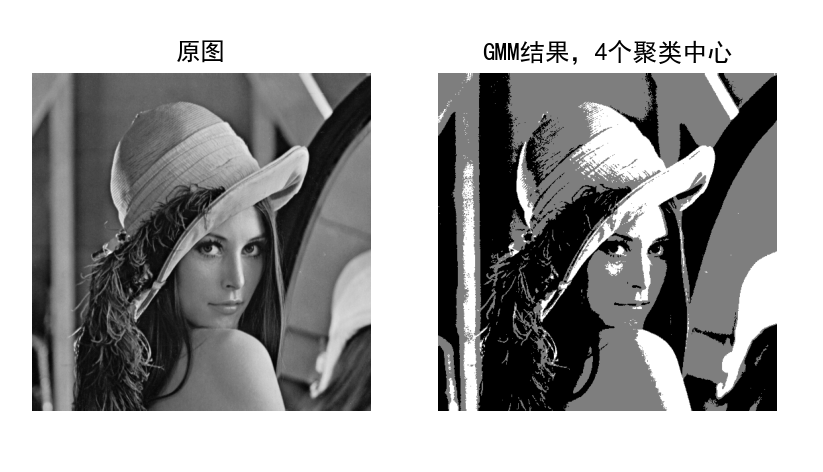
\includegraphics[scale=1]{3.png}
\end{figure}

\section*{二、图像分割算法拓展}	
\section{FCM聚类算法}
\subsection{理论知识}
模糊C均值聚类(Fuzzy C-Means), 简称FCM,是一种引入模糊理论的聚类算法。因为在许多情况下多个类别界限并不绝对,在该算法中,我们引入隶属度用来表示一个样本属于某一类的概率。相比于Kmeans聚类方法,FCM得到的聚类结果更加灵活。

最小化目标函数为:
$$ J=\sum_{i=1}^c \sum_{j=1}^nu_{ij}^m\|x_j-c_i\|^2\qquad(1)$$
约束条件为:
$$\sum_{i=1}^{c}u_{ij}=1\, j=1,2,\cdots n\ \qquad(2)$$
其中c表示聚类中心个数,n为样本个数,m是一个隶属度的因子,可取2,3等值,表示样本属不属于某类的重要程度。$u_{ij}$表示样本j对于类i的隶属度。由(1)知,目标函数由相应样本的隶属度与该样本到各个类中心的距离相乘组成。约束条件(2)表示样本对各个类隶属度之和要为1。

要让目标函数取得最小值,我们使用拉格朗日乘数法将约束条件放入目标函数中,得到:
$$J=\sum_{i=1}^c \sum_{j=1}^nu_{ij}^m\|x_j-c_i\|^2+\lambda_1(\sum_{i=1}^{c}u_{i1}-1)+\cdots+\lambda_n(\sum_{i=1}^{c}u_{in}-1)\qquad$$
分别对$u_{ij},c_i$求导可以得到:
$$c_i=\frac{\sum_{j=1}^n(u_{ij}^mx_j)}{\sum_{j=1}^nu_{ij}^m}\ \ \quad\qquad\qquad(3)$$
$$u_{ij}=\frac{1}{\sum_{k=1}^{c}(\frac{\|x_j-c_i\|}{\|x_j-c_k\|})^{(\frac{2}{m-1})}}\qquad(4)$$
(3)是类中心的迭代公式,(4)是隶属度矩阵的迭代公式,我们可以随机初始化满足约束条件的隶属度矩阵,然后通过公式迭代,得到FCM的分类结果。

\subsection{代码结构}
\subsubsection{初始化隶属度矩阵U}
\begin{python}
	def Initial_U(sample_num, cluster_n):
		 # sample_num为样本个数, cluster_n为分类数
		 U = np.random.rand(cluster_n,sample_num)
		 # 对 U 按列求和,然后取倒数
		 col_sum = np.sum(U, axis=0)
		 col_sum = 1 / col_sum
		 # 确保 U 的每列和为1
		 U = np.multiply(U, col_sum)
		 return U
\end{python}	
\subsubsection{计算更新类中心}
\begin{python}
	def Cen_Iter( data, U, cluster_n):
		 # 初始化中心点
		 center = np.zeros(cluster_n)
		 for i in range(0, cluster_n):
		 	  # 根据迭代公式进行计算
			  u_ij_m = U[i, :] ** m
			  sum_u = np.sum(u_ij_m)
			  # 矩阵乘法
			  ux = np.dot(u_ij_m, data)
			  center[i] =  ux / sum_u
	 	 return center
\end{python}	
\subsubsection{计算更新隶属度矩阵}
\begin{python}
	def U_Iter(data,U, c):
		 cluster_n,sample_num = U.shape
		 for i in range(0, cluster_n):
		 	 for j in range(0,sample_num):
		 	 	 sum = 0
		 	 	 # 根据隶属度矩阵迭代公式计算
		 	 	 for k in range(0, cluster_n):
		 	 	 	 temp = (np.linalg.norm(data[j] - c[i]) /
		 	 	 	 np.linalg.norm(data[j] - c[k])) ** (2 / (m - 1))
		 	 	 	 sum = temp + sum
		 	 	 U[i, j] = 1 / sum
		 return U
\end{python}	
\subsubsection{图片分割与可视化}
\begin{python}
	def FCM(img_path,cluster_n=5,iter_num=10): # 迭代次数默认为10
		 # 读入灰度图像
		 img=cv2.imread(img_path,0)
		 # 将图片拉成一列
		 data=img.reshape(img.shape[0]*img.shape[1],1)
		 sample_num = len(data)
		 # 初始化隶属度矩阵U
	 	 U = Initial_U(sample_num, cluster_n)
		 for i in range(0, iter_num):
		 	 C = Cen_Iter(data, U, cluster_n)
		 	 U = U_Iter(data,U, C)	 	 
		 # 分类标签
		 label = np.argmax(U, axis=0)
		 # 最后的类中心矩阵
		 center = C
		 # 根据聚类结果和聚类中心构建新图像
		 new_img=center[label]
		 # 矩阵转成原来图片的形状
		 new_img=np.reshape(new_img,img.shape)
		 # 要变成图像得数据得转换成uint8
		 new_img=new_img.astype('uint8')
		 plt.subplot(121),plt.imshow(img, cmap="gray")
		 plt.title("原图"),plt.axis('off')
		 plt.subplot(122),plt.imshow(new_img, cmap="gray")
		 plt.title("FCM,%d个聚类中心"%cluster_n),plt.axis('off')
		 plt.show()
\end{python}	
运行结果如下:
\begin{figure}[H]  
	\centering
	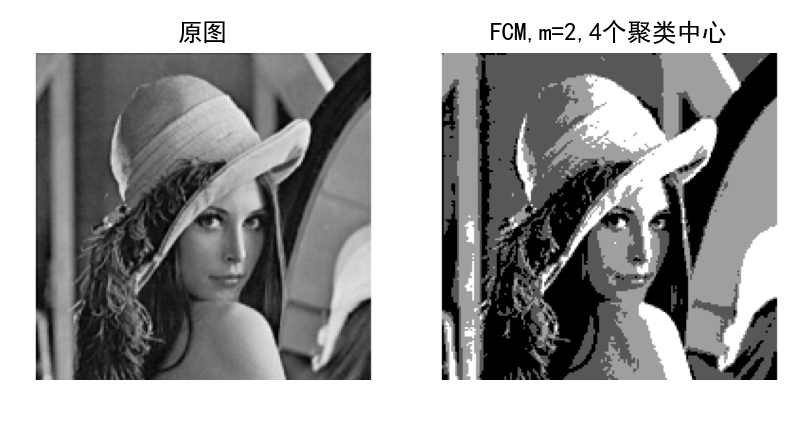
\includegraphics[scale=1]{1.png}
	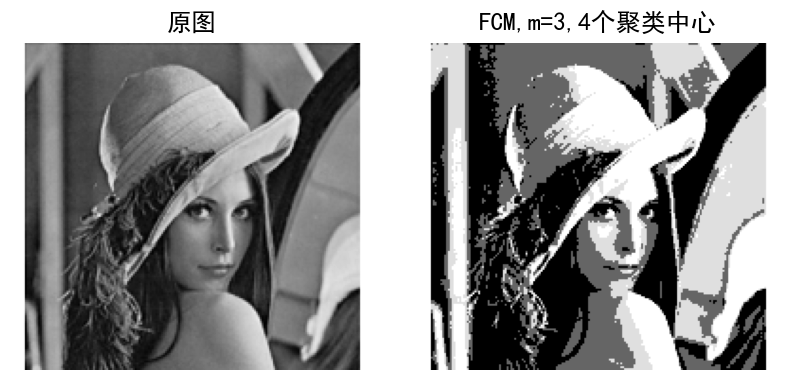
\includegraphics[scale=1]{2.png}
\end{figure}	


我们可以看到FCM算法图像分割效果还不错,适用于图像中存在不确定性和模糊性;但其分割速度较慢,没有考虑空间信息,对噪声和灰度不均匀敏感。

\subsection{代码优化}

当我们确定$m=2$时,可以通过使用矩阵乘法代替for循环的方法加快运行时间,具体优化代码如下:
\subsubsection{计算更新类中心}
\begin{python}
	def Cen_Iter(data, U):
		 U_m = U**2
		 sum_u = np.sum(U_m, axis=1)
		 ux = np.sum(np.dot(U_m, data), axis=1)
		 center = np.true_divide(ux, sum_u)
		 return center
\end{python}

\subsubsection{计算更新隶属度矩阵}
\begin{python}
	def U_Iter(data, U, c):
		 cluster_n,sample_num = U.shape
		 data2_trans = (data**2).reshape((1,sample_num))
		 c2_trans = (c**2).reshape((cluster_n,1))
		 dist1 = np.dot(np.ones((cluster_n,1)), data2_trans) + \
		 	 	 	np.dot(c2_trans, np.ones((1, sample_num))) - 2*np.dot(c.reshape((cluster_n,1)), data.T)
		 dist2 = np.true_divide(np.ones(U.shape),dist1)
		 sum_k = np.sum(dist2, axis=0)
		 U = np.multiply(dist1, sum_k)
		 U = np.true_divide(np.ones(U.shape), U)
		 return U
\end{python}	

优化后运行时间可以从120秒变成2秒,优化效果非常显著。

\section{SCA聚类算法}
\subsection{基本概念}
SCA( Sine Cosine Algorithm)算法是一种新颖的全优化算法,它基于数学中正弦/余弦函数图像的概念,使最佳解可以向内或向外扩展,而且算法本身拥有勘探和开发两个阶段,可以对最佳位置进行深度挖掘,最终达到全局最优的目的。

我们将K-均值聚类算法和SCA优化算法结合,即将K-均值方法的结果作为一个正余弦因子并采用正余弦优化的方法,通过适应度函数,利用新的分类中心调整粒子位置,产生新的聚类中心.并将此方法应用于图像的分割。

\subsection{算法实现}

\textbf{1、初始化:}

初始化所有参数,包括搜索智能体数目$N$,最大迭代次数$T$,$r_1$和随机因子$r_2,r_3,r_4$,并提供初始化解空间$x_i(i=1,2\cdots,N)$。

\textbf{2、计算所有解的适应度:}

将每个解带入目标函数进行计算。

\textbf{3、更新$r_1$和解的位置}

$$r_1=a-t\frac{a}{T}$$
$a$是一个常数; $t$ 为当前迭代次数; $T$为最大迭代次数。参数$r_1$表示下一个解的位置区域在当前解和最优解之内或者之外,较小的$r_1$有助于增强算法的局部开发能力,较大的$r_1$有助于提高算法的全局探索能力,同时 $r_1$的值随迭代次数逐渐减小,平衡了算法局部开发和全局搜索的能力。

$$X_i^{t+1}=\begin{cases}
	X_i^t+r_1*\sin(r_2)*|r_3P_i^t-X_i^t|\qquad r_4<0.5\\
	X_i^t+r_1*\cos(r_2)*|r_3P_i^t-X_i^t|\qquad r_4>0.5\
\end{cases}$$

$X_i^t$是当前个体的第$i$维第$t$次迭代的位置;$r_2$为0到$2\pi$的随机数,
定义了当前解朝向或者远离最优解多远;$r_3$为0到2之间的随机数,为最优解给出一个随机权重值,是为了随机强调( $r_3 >1 $)或者忽略($r_3 <1 $)最优解在定义候选解移动距离时的影响效果;$r_4$为0到1的随机数,平等地切换正弦和余弦函数。$P_i^t$表示在$t$次迭代时最优个体第$i$维的位置。

\textbf{4、比较并更新全局最优解的位置:}

将更新后的每一个解的适应度值与全局最优解的适应度值进行比较,如果当前解的目标函数小于全局最优的目标函数,则更新全局最优解的位置。

\textbf{5、算法终止:}

重复(2)-(4)的步骤,当满足预定义的迭代次数时,算法停止。

\subsection{代码结构}
\subsubsection{初始化SCA算法聚类问题类}
\begin{python}
	class SCA:
		 # 用正弦余弦算法解决聚类问题
		 def __init__(self, image, k, agent_num, max_iters):
		 """
		 初始化
		 :param image: 输入的图像
		 :param k: 聚类的数目
		 :param agent_num: 搜索智能体的数目
		 :param max_iters: 最大迭代次数
		 """
		 self.image = image
		 self.shape = image.shape  # 图像大小
		 # 为阈值设定界限
		 self.low_bound = 0
		 self.upper_bound = 255
		 self.k = k
		 self.agent_num = agent_num
		 self.max_iters = max_iters
		 # 包含所有智能体位置的矩阵
		 self.X = np.zeros((self.agent_num, self.k))
		 # 存储目标函数值
		 self.obj_values = [0.0] * self.agent_num
		 # 初始化
	 	 self.initialization()
		 self.fitness()
		 # 最优
		 self.P = None
\end{python}
\subsubsection{搜索智能体初始化}
\begin{python}
	def initialization(self):
		 """
		 初始化搜索智能体
		 :return:
		 """
		 # 包含所有智能体位置(阈值)的矩阵
		 X = np.random.randint(self.low_bound, self.upper_bound+1, size=(self.agent_num,self.k), dtype='int32')
		 self.X = X
		 return X
\end{python}
\subsubsection{目标函数}
\begin{python}
	def fitness(self):
		 """
		 求目标函数
		 :param x:
		 :return:
		 """
		 for i in range(self.agent_num):
		 	 x = self.X[i, :]
		 	 m, n = self.shape
		 	 image_list = [self.image.reshape(m*n)] * self.k
		 	 images = np.stack(image_list, axis=1)
		 	 value = np.sum((images - x) ** 2)
		 	 self.obj_values[i] = value
\end{python}
\subsubsection{寻找最优位置}
\begin{python}
	def search(self):
		 """
		 迭代寻找最优
		 :return:
		 """
		 # 更新
		 for iter in range(1,self.max_iters):
		 	 self.P = self.X[np.argmin(self.obj_values), :]
		 	 # update r1
		 	 a = 2
		 	 r_1 = a - iter * a / self.max_iters
		 	 # update r2,r3,r4
		 	 r_2 = 2 * np.pi * np.random.rand(self.agent_num, self.k)
		 	 r_3 = 2 * np.random.rand(self.agent_num, self.k)
		 	 r_4 = np.random.rand(self.agent_num, self.k)
		 	 # update positions of X
		 	 boolmatrix = r_4 < 0.5
		 	 add_sin = r_1 * np.sin(r_2) * np.abs(r_3 * self.P - self.X) * boolmatrix
		 	 add_cos = r_1 * np.cos(r_2) * np.abs(r_3 * self.P - self.X) * (1 - boolmatrix)
		 	 self.X += add_sin.astype('int32')
		 	 self.X += add_cos.astype('int32')
		 	 # 边界检查(截断)
		 	 low_judge = self.X < self.low_bound
		 	 self.X = self.X * (1 - low_judge) + low_judge * self.low_bound
		 	 upper_judge = self.X > self.upper_bound
		 	 self.X = self.X * (1 - upper_judge) + upper_judge * self.upper_bound
		 	 # 更新 obj_values
		 	 self.fitness()
\end{python}
\subsubsection{图像分割}
\begin{python}
	def threshold_seg(self):
		 """
		 根据阈值进行图像分割
		 :return: new_image 分割之后的图像 ndarray
		 """
		 new_image = np.zeros(self.shape, dtype='int32')
		 # 选择最小目标函数
		 threshold_list = list(self.X[np.argmin(self.obj_values), :])
		 threshold_list.sort()
		 threshold_list.append(255)
		 # k 阈值分类
		 for i in range(self.k+1):
		 	 if i == 0:
		 	 	 judge1 = self.image >= 0
		 	 	 judge2 = self.image < threshold_list[i]
		 	 	 new_image += threshold_list[i] * judge1 * judge2
	  		else:
		 	 	 judge1 = self.image >= threshold_list[i-1]
		 	 	 judge2 = self.image < threshold_list[i]
		 	 	 new_image += threshold_list[i] * judge1 * judge2
		 return new_image
\end{python}

\section{GA算法}

\subsection{基本概念}
遗传算法(GA)是一种模拟基因的元启发式算法,它模拟了自然选择和自然遗传过程中发生的繁殖、交配和突变现象。GA是一个基于种群(population)的算法(即每次迭代产生多个解)。每次迭代的解的个数称为种群大小。每个解用染色体表示,每一条染色体都是由基因组成。

对于一个种群大小为n的遗传算法,是从n个随机解开始。然后,选择最优解杂交产生新的解。将产生的最优解添加到下一个迭代中,并舍弃不好的结果。不断进行迭代,可以实现将这些解在一定程度上收敛至接近最优解。

我们利用遗传算法解决OTSU多阈值算法,将k个阈值按顺序排列起来构成一条基因串:
$$\alpha=\{T_1,T_2,\cdots,T_k\}$$
由于灰度值范围为0-255,我们可以使用8位二进制代码表示每个阈值,此时每个基因串由长度为$8\times k$个bit位的数组组成。我们采用OTSU计算的类间方差作为适应度函数,类间方差越大,适应度函数值就越高。
\subsection{算法实现}
\textbf{1、种群初始化:}

将基因设置为随机值,创造n条染色体作为第一代解。

\textbf{2、适应度评估:}

用适应度函数评价每条染色体的适应度。

\textbf{3、选择:}

根据适应度函数的大小随机淘汰个体(染色体)。

\textbf{4、交叉:}

遍历种群中的每一个个体,将该个体作为父亲,随机选择另一个体,并将该个体作为母亲,随机产生交叉的点,孩子得到位于交叉点后的母亲的基因。

\textbf{5、变异:}

交叉可能陷入局部最优。为了克服该问题,随机选择的一个基因进行突变操作,通过在染色体上随机翻转一个bit来完成变异。

\textbf{6、终止:}

重复(2)-(5)的步骤,当满足预定义的迭代次数时,遗传算法就停止。


\subsection{代码结构}

\subsubsection{初始化遗传算法图像分割类}

\begin{python}
	class GA_seg:
    # 用遗传算法解决OTSU多阈值算法
    def __init__(self, image, k=4, pop_size=30, p_mutation=0.3, p_cross=0.8, max_iters=200):
        """
        初始化遗传算法图像分割类
        :param image: 输入图像 ndarray
        :param k: 分类的数目 int
        :param pop_size: 种群大小 int
        :param p_mutation: 染色体发生变异的概率 float
        :param p_cross: 染色体发生交叉的概率 flaot
        :param max_iters: 最大迭代次数 int
        """
        self.image = image
        self.shape = image.shape  # 图像大小
        # 直方图
        m,n = self.shape
        self.hist = nD_histogram(self.image.reshape((m*n, 1)), 1, [256], [0], [256])
        self.k = k-1  # 分成k类需要k-1个阈值
        self.pop_size = pop_size
        self.gene_length = 8  # 染色体中每个基因的长度,8bit二进制数可以表示[0,255]
        self.populations = self.initial_encode()
        self.p_mutation = p_mutation
        self.p_cross = p_cross
        self.fitvalue = np.array([1e-3] * self.pop_size)
        self.max_iters = max_iters
\end{python}
\subsubsection{种群初始化}
\begin{python}
    def initial_encode(self):
        """
        初始随机编码出染色体
        :return: chromosomes 所有编码出的染色体个体 ndarray(size=self.pop_size*self.k*8)
        """
        m,n = self.shape
        # 图像中的所有坐标
        x_coords = np.arange(m)
        y_coords = np.arange(n)
        # # 初始化时随机选取self.pop_size*self.k个坐标
        rand_chos_x = np.random.choice(x_coords, size=self.pop_size * self.k, replace=True)  # 初始化时随机选取的坐标
        rand_chos_y = np.random.choice(y_coords, size=self.pop_size * self.k, replace=True)
        # 存储
        chromosomes = []
        for i in range(self.pop_size):
            # 编码 将所有阈值用二进制表示成基因,所有基因构成染色体
            ind_code = ''
            for j in range(self.k):
                code_str = bin(self.image[rand_chos_x[i*self.k+j], rand_chos_y[i*self.k+j]])[2:]
                if len(code_str) < 8:
                    code_str = '0' * (8 - len(code_str)) + code_str
                ind_code += code_str
                # ind_code += self.image[rand_chos_x[i*self.k+j], rand_chos_y[i*self.k+j]] << 8 * j
            # code_str = bin(ind_code)[2:]
            # 统一编码得到长度为8*self.k的基因
            assert len(ind_code) == 8 * self.k  # 检验是否编码成功
            # print(code_str)
            code = np.array(list(map(int,list(ind_code))))
            chromosomes.append(code)
        return np.array(chromosomes)
\end{python}
\subsubsection{适应度函数}
\begin{python}
    def fitness(self):
        """
        计算适应度函数:采用OTSU计算类间方差
        :return: f_list 不同染色体个体的适应度函数
        """
        start = time.time()
        L = 256
        m, n = self.shape
        N = m * n
        # 图片的概率直方图
        imhist = self.hist/N
        standn = np.arange(L)
        # 图片的全局像素平均值
        mu_g = np.sum(standn * self.hist) / N
        # 适应度函数 f_list
        f_list = [0.0] * self.pop_size  # pop_size 是可变的
        for i in range(self.pop_size):
            # 每一个染色体
            chromosome = self.populations[i, :]
            # 解码为阈值数组
            threshold_list = self.decode(chromosome)
            threshold_list.append(256)
            # 计算类间方差
            for j in range(self.k):
                if j == 0:
                    w = np.sum(imhist[0:threshold_list[j]])
                    if w > 0:
                        mu = np.dot(imhist[0:threshold_list[j]], np.arange(0,threshold_list[j])) / w
                        f_list[i] += w * (mu - mu_g) ** 2
                else:
                    w = np.sum(imhist[threshold_list[j]:threshold_list[j+1]])/N
                    if w > 0:
                        mu = np.dot(imhist[threshold_list[j]:threshold_list[j+1]],
                                            np.arange(threshold_list[j],threshold_list[j+1])) / w
                        f_list[i] += w * (mu - mu_g) ** 2
        end = time.time()
        # print(end - start)  # 打印运行时间
        self.fitvalue = np.array(f_list)
        return f_list
\end{python}
\subsubsection{选择}
\begin{python}
    def selection(self):
        """
        物竞天择,淘汰选择个体
        """
        # 根据适应度函数的大小随机淘汰个体
        # idx = np.random.choice(np.arange(self.pop_size), size=int(self.pop_size*4/5), replace=True,
        #                        p=(self.fitvalue) / (self.fitvalue.sum()))
        idx = np.random.choice(np.arange(self.pop_size), size=int(self.pop_size), replace=True,
                               p=(self.fitvalue) / (self.fitvalue.sum()))
        self.populations = self.populations[idx]
        self.pop_size = self.populations.shape[0]
\end{python}
\subsubsection{交叉}
\begin{python}
    def crossover(self):
        """
        染色体的交叉
        """
        for i in range(self.pop_size):
            father = self.populations[i, :].copy()  # 遍历种群中的每一个个体,将该个体作为父亲
            child = father  # 孩子先得到父亲的全部基因
            if np.random.rand() < self.p_cross:  # 以p_cross的概率进行变异
                mother = self.populations[np.random.randint(self.pop_size), :].copy()  # 随机选择另一个体,并将该个体作为母亲
                cross_points = np.random.randint(0, self.k*8)  # 随机产生交叉的点
                child[cross_points:] = mother[cross_points:]  # 孩子得到位于交叉点后的母亲的基因
            self.populations[i, :] = child  # 替代父亲
            # new_populations = np.zeros((self.pop_size+1, self.k*8), dtype='int32')
            # new_populations[:self.pop_size, :] = self.populations
            # new_populations[self.pop_size, :] = child
            # self.populations = new_populations  # 遗传
            # self.pop_size += 1
\end{python}
\subsubsection{变异}
\begin{python}
    def mutation(self):
        """
        染色体的变异
        """
        for i in range(self.pop_size):
            if np.random.rand() < self.p_mutation:  # 以p_mutation的概率进行变异
                mutate_point = np.random.randint(0, self.k*8)  # 随机产生一个实数,代表要变异基因的位置
                self.populations[i, mutate_point] ^= 1  # 将变异点的二进制为反转
\end{python}
\subsubsection{终止}
\begin{python}
	def train(self):
		 # 初始化种群
		 self.initial_encode()
		 # 初始化适应度函数
		 self.fitness()
		 for iter in range(self.max_iters):
		 	 # 选择
		 	 self.selection()
		 	 # 交叉
		 	 self.crossover()
		 	 # 变异
		 	 self.mutation()
		 	 # 求适应度函数
		 	 self.fitness()
	  	 	 return self.threshold_seg()
\end{python}
\section{PSO算法}
\subsection{基本概念}
\textbf{粒子群优化算法}(Particle Swarm Optimization)是进化算法的一种,它源于鸟群捕食的行为研究,基本思想是通过群体中个体之间的协作和信息共享来寻找最优解。在PSO中,每个优化问题的潜在解都是搜索空间中的一只鸟,抽象为粒子。

所有粒子都在一个d维空间进行搜索,由目标函数来确定适应值以判断目前的位置好坏。每一个粒子被赋予记忆功能,能记住所搜寻到的最佳位置。每一个粒子还有一个速度以决定飞行的距离和方向。这个速度根据它本身的飞行经验以及同伴的飞行经验进行动态调整。

\subsection{算法实现}
\textbf{1、初始化:}

初始化粒子群,给每个粒子赋予随机的初始位置和速度。

\textbf{2、计算适应值:}

根据适应度函数,计算每个粒子的适应值。

\textbf{3、求个体最佳适应值:}

对每个粒子,将其当前位置适应值与其历史最佳位置对应适应值比较,若当前位置适应值更高,则用当前位置更新历史最佳位置。

\textbf{4、求全局最佳适应值:}

对每一个粒子,将其当前位置适应值与其全局最佳位置对应适应值比较,如果当前位置的适应值更高,则用当前位置更新全局最佳位置。

\textbf{5、更新粒子位置和速度:}

根据公式更新每个粒子的速度与位置。

速度更新公式:
$$v_i(t+1)=\alpha v_i(t)+\beta_1r_1(pbest_i(t)-x_i(t))+\beta_2r_2(gbest(t)-x_i(t))$$
位置更新公式:
$$x_i(t+1)=x_i(t)+v_i(t+1)$$
上面公式中:$i$表示粒子编号;$t$表示时刻,反映在迭代次数上;$\alpha$是惯性权重,一般设置在0.4左右;$\beta_1,\beta_2$表示学习因子,一般都取值为2;$pbest_i$表示的是粒子$i$的经验,也即是粒子$i$所到过最佳位置;$gbest$代表的是全局最优粒子的位置;$r_1,r_2$是0到1之间的随机值。

\textbf{6、判断算法是否结束:}

通常算法达到最大迭代次数或者最佳适应度值的增量小于某个给定的阈值时算法停止。

\subsection{代码结构}

\subsubsection{初始化粒子群算法图像分割类}
\begin{python}
	class PSO:
    def __init__(self, image, k=4, pop_size=30, max_iters=200, w=0.72, c1=1.49, c2=1.49):
        """
        初始化
        :param image: 输入图像 ndarray
        :param k: 分类的数目 int
        :param pop_size: 种群的大小 int
        :param max_iters: 最大迭代次数 int
        :param w: 惯性权重因子 float
        :param c1: 加速因子 float
        :param c2: 加速因子 float
        """
        self.image = image
        self.shape = image.shape  # 图像大小
        # 直方图
        m, n = self.shape
        self.hist = nD_histogram(self.image.reshape((m * n, 1)), 1, [256], [0], [256])
        self.k = k-1  # 分成k类需要k-1个阈值
        self.pop_size = pop_size
        self.max_iters = max_iters
        self.w = w
        self.c_1 = c1
        self.c_2 = c2
        # 为粒子位置、速度设定界限
        self.X_lower = 0
        self.X_upper = 255
        self.v_lower = -4.0
        self.v_upper = 4.0
        # 包含所有粒子位置(阈值)的矩阵
        self.X = np.zeros((self.pop_size, self.k), dtype='int32')
        # 包含所有粒子速度的矩阵
        self.v = np.zeros((self.pop_size, self.k))
        # 存储目标函数值
        self.fitvalue = np.array([0.0] * self.pop_size)
        self.initialization()
        # 存储全局最优和局部最优
        self.pbest = self.X
        self.pbestvalues = np.zeros(self.pop_size)
        self.gbest = self.X[0, :]
        self.gbestvalue = 0
\end{python}

\subsubsection{初始化粒子群的位置和速度}
\begin{python}
    def initialization(self):
        """
        随机初始化粒子群的位置和速度
        """
        self.X = np.random.randint(self.X_lower, self.X_upper+1, size=(self.pop_size,self.k), dtype='int32')
        self.v = np.random.randint(self.v_lower, self.v_upper+1, size=(self.pop_size,self.k))
        self.fitness()
        self.get_initbest()
\end{python}

\subsubsection{适应度函数}
\begin{python}
    def fitness(self):
        """
        计算适应度函数:采用OTSU计算类间方差
        :return: f_list 不同染色体个体的适应度函数
        """
        L = 256
        m, n = self.shape
        N = m * n
        # 图片的概率直方图
        imhist = self.hist / N
        standn = np.arange(L)
        # 图片的全局像素平均值
        mu_g = np.sum(standn * self.hist) / N
        # 适应度函数 f_list
        f_list = [0.0] * self.pop_size  # pop_size 是可变的
        for i in range(self.pop_size):
            # 阈值数组
            threshold_list = list(self.X[i, :])
            threshold_list.append(256)
            # 计算类间方差
            for j in range(self.k):
                if j == 0:
                    w = np.sum(imhist[0:threshold_list[j]])
                    if w > 0:
                        mu = np.dot(imhist[0:threshold_list[j]], np.arange(0, threshold_list[j])) / w
                        f_list[i] += w * (mu - mu_g) ** 2
                else:
                    w = np.sum(imhist[threshold_list[j]:threshold_list[j + 1]]) / N
                    if w > 0:
                        mu = np.dot(imhist[threshold_list[j]:threshold_list[j + 1]],
                                    np.arange(threshold_list[j], threshold_list[j + 1])) / w
                        f_list[i] += w * (mu - mu_g) ** 2
        # print(end - start)  # 打印运行时间
        self.fitvalue = np.array(f_list)
        return f_list
\end{python}

\subsubsection{获得局部和全局最优适应值}
\begin{python}
    def get_initbest(self):
        """
        获得局部和全局最优位置
        """
        self.gbest = self.X[self.fitvalue.argmax(), :].copy()
        self.gbestvalue = self.fitvalue.max()
        self.pbest = self.X.copy()
        self.pbestvalues = self.fitvalue.copy()
\end{python}

\subsubsection{迭代优化}
\begin{python}
    def run(self):
        """
        迭代优化
        """
        # 迭代优化
        for i in range(self.max_iters):
            # 速度更新
            self.v = self.w * self.v + \
                     self.c_1 * np.random.rand(self.pop_size,self.k) * (self.pbest - self.X) + \
                self.c_2 * np.random.rand(self.pop_size,self.k) * (self.gbest - self.X)
            # 防止越界 截断处理
            lower_judge = self.v < self.v_lower
            self.v = self.v * (1 - lower_judge) + lower_judge * self.v_lower
            upper_judge = self.v > self.v_upper
            self.v = self.v * (1 - upper_judge) + upper_judge * self.v_upper
            # 粒子位置更新
            self.X += self.v.astype('int32')
            # 防止越界 截断处理
            lower_judge = self.X < self.X_lower
            self.X = self.X * (1 - lower_judge) + lower_judge * self.X_lower
            upper_judge = self.X > self.X_upper
            self.X = self.X * (1 - upper_judge) + upper_judge * self.X_upper
            # 适应度函数更新
            self.fitness()
            # pbest,gbest 更新
            for j in range(self.pop_size):
                if self.fitvalue[j] > self.pbestvalues[j]:
                    self.pbestvalues[j] = self.fitvalue[j]
                    self.pbest[j, :] = self.X[j, :].copy()
            if self.gbestvalue < self.pbestvalues.max():
                self.gbestvalue = self.pbestvalues.max()
                self.gbest = self.X[self.pbestvalues.argmax()].copy()

        return self.gbest, self.gbestvalue
\end{python}



%& Population size & Max iterations
\section{实验结果和讨论}
%-------------------------------------------------
\subsection{正弦余弦算法(SCA)}

使用正弦余弦算法(SCA)进行聚类,我们的超参数设置如下:
\begin{table}[h]
	\centering
	\begin{tabular}{cccc}
	  \hline
	  Cluster numbers(k) & r1,r2,r3,r4 & Population size & Max iterations\\ \hline
	  4
	  & random numbers
	  & 30
	  & 200
	  \\ \hline
	\end{tabular}
	\caption{Hyper parameter description}
\end{table}

固定超参数,进行五次实验,得到结果如下所示:

\begin{figure*}[h]
	\begin{minipage}[t]{0.2\textwidth}%并排放两张图⽚,每张占页⾯的0.5,下同。
		\centering
		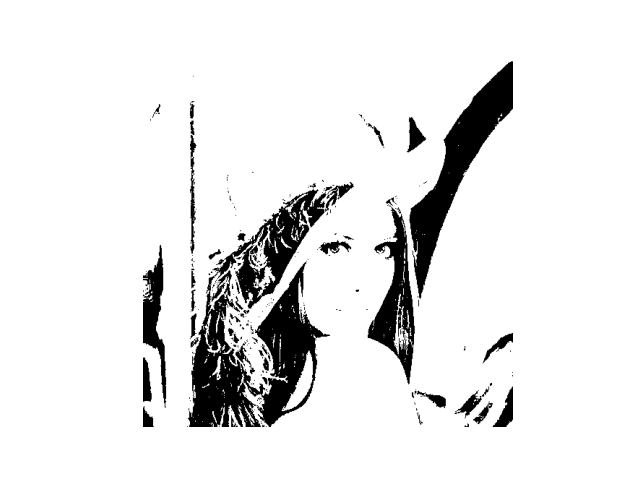
\includegraphics[width=\textwidth]{SCA_1.png}
		\caption{Case1}%注释1.jpg
		\end{minipage}
	\begin{minipage}[t]{0.2\textwidth}
		\centering
		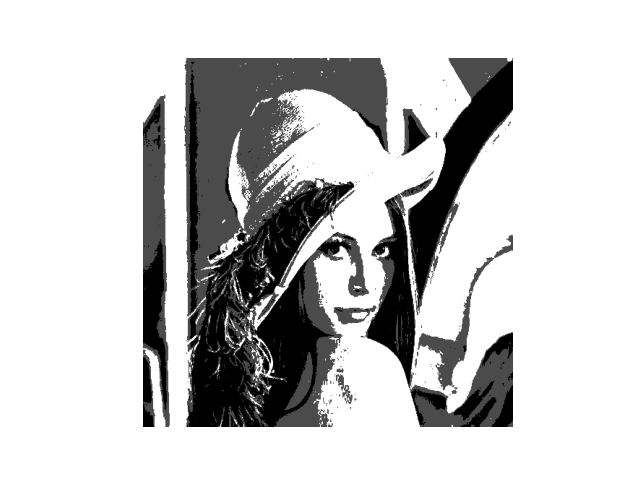
\includegraphics[width=\textwidth]{SCA_2.png}
		\caption{Case2}
	\end{minipage}
	\begin{minipage}[t]{0.2\textwidth}
		\centering
		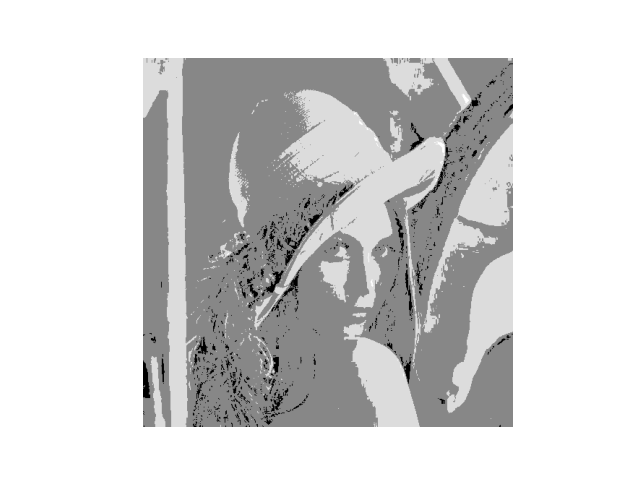
\includegraphics[width=\textwidth]{SCA_3.png}
		\caption{Case3}
	\end{minipage}
	\begin{minipage}[t]{0.2\textwidth}
		\centering
		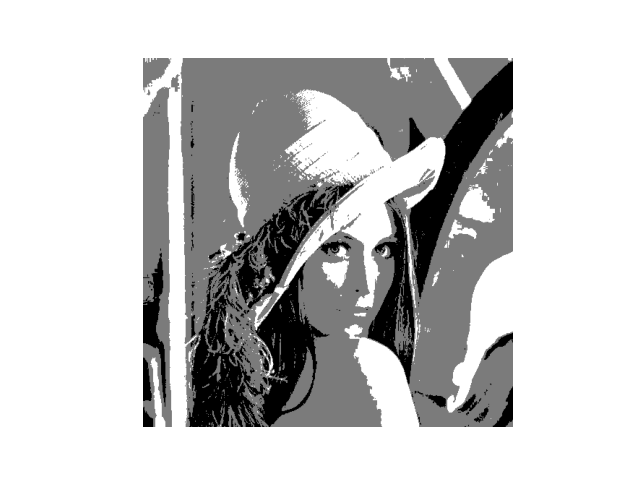
\includegraphics[width=\textwidth]{SCA_4.png}
		\caption{Case4}
	\end{minipage}
\end{figure*}

SCA算法也是随机算法,结果同样不稳定。另外,从结果中可以看出,我们的SCA算法并不能得到很好的效果。由于SCA算法中,目标函数的选择十分重要,我们考虑有可能设计出比论文中更合适的目标函数来得到更好的结果。

%-------------------------------------------------
\subsection{遗传算法(GA)}
使用遗传算法(GA)求解OTSU多阈值问题,我们的超参数设置如下:
\begin{table}[h]
	\centering
	\begin{tabular}{ccccc}
	  \hline
	  Cluster numbers(k) & Crossover probablity & Mutation probablity & Population size & Max iterations\\ \hline
	  4
	  & 0.8
	  & 0.3
	  & 30
	  & 200
	  \\ \hline
	\end{tabular}
	\caption{Hyper parameter description}
\end{table}

固定超参数,进行五次实验,得到结果如下所示:

\begin{figure*}[h]
	\begin{minipage}[t]{0.2\textwidth}%并排放两张图⽚,每张占页⾯的0.5,下同。
		\centering
		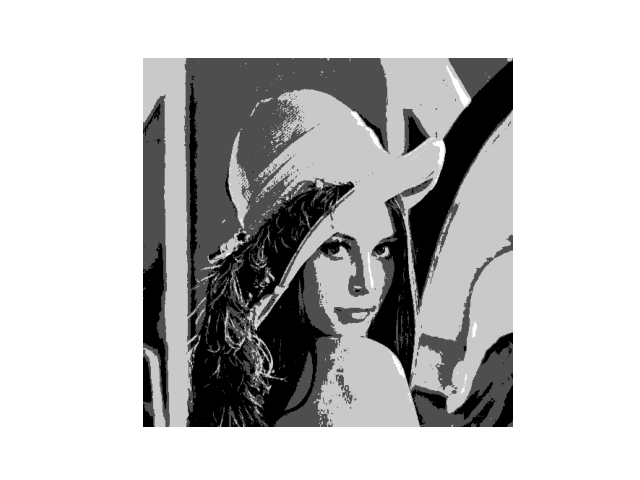
\includegraphics[width=\textwidth]{GA_1.png}
		\caption{Case1}%注释1.jpg
		\end{minipage}
	\begin{minipage}[t]{0.2\textwidth}
		\centering
		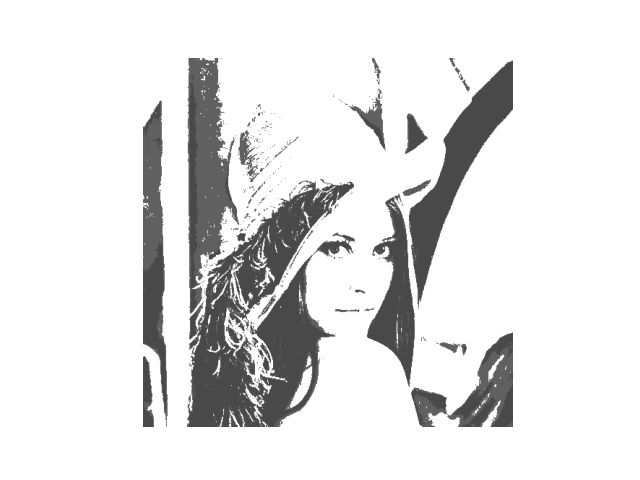
\includegraphics[width=\textwidth]{GA_2.png}
		\caption{Case2}
	\end{minipage}
	\begin{minipage}[t]{0.2\textwidth}
		\centering
		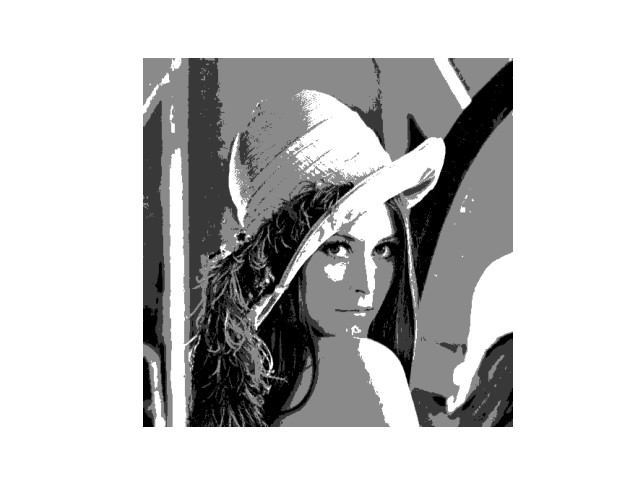
\includegraphics[width=\textwidth]{GA_3.png}
		\caption{Case3}
	\end{minipage}
	\begin{minipage}[t]{0.2\textwidth}
		\centering
		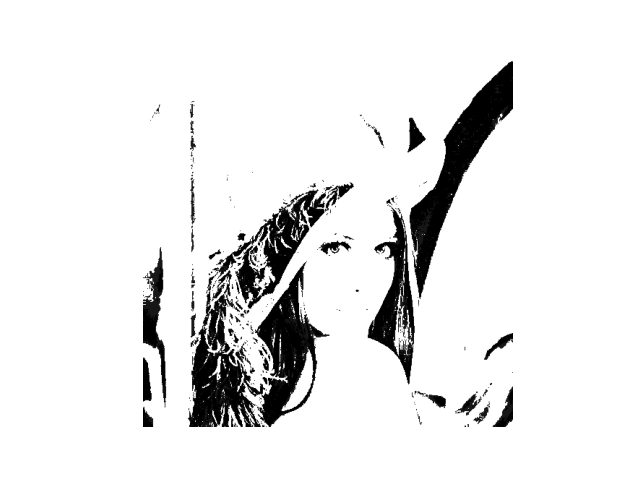
\includegraphics[width=\textwidth]{GA_4.png}
		\caption{Case4}
	\end{minipage}
	\begin{minipage}[t]{0.2\textwidth}
		\centering
		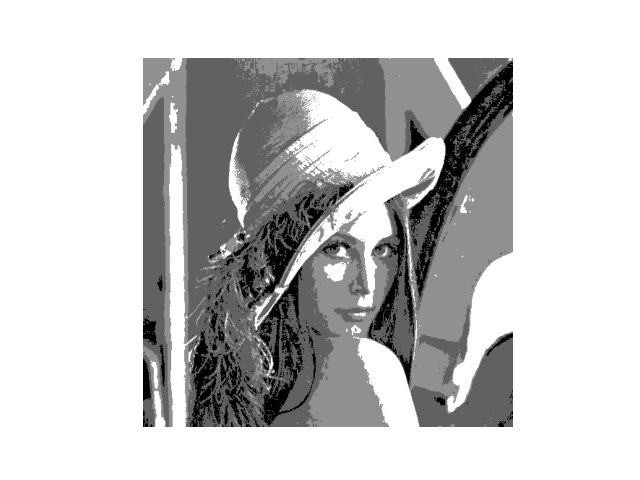
\includegraphics[width=\textwidth]{GA_5.png}
		\caption{Case5}
	\end{minipage}
\end{figure*}

可以发现,利用遗传算法求OTSU多阈值问题,能够很快得到结果,大大减少了多阈值OTSU遍历全部阈值数组所需要的时间。但由于遗传算法是随机算法,其图像分割效果很不稳定,随着迭代次数的增加,其会逐渐逼近局部最优值甚至全局最优值,但一方面不能保证达到全局最优值,另一方面由于存在变异过程,达到最优值后也可能因为变异而是结果产生波动。我们思考或许可以随着迭代过程逐步改变变异和遗传的概率,从而使我们的结果更加稳定。
\subsubsection*{GA算法优化}
经过分析,另外的问题在于,在遗传算法的种群初始化步骤中,个体分布通常不均匀,某些区域不会分配个体搜索,从而导致错过全局最优解或陷入局部最优解。而如果人工控制初始化使其分布均匀,又可能导致大量个体在远离全局最优解的位置搜索,从而减缓进化速度。

查阅论文可知,可以使用经验遗传算法(EGA)加以改进。其种群初始化分为两步,首先均匀分配初始种群进行统一搜索,在一定的搜索步数后停止,而后对结果较好的区域分配更多的个体进行重点搜索,提高后期的搜索效率。与经典的遗传算法相比,EGA可以控制个体进化的方向,从而在高效率的同时保证找到全局最优解。该方法在图像处理及时间序列预测等领域均已被广泛应用。

%-------------------------------------------------
\subsection{粒子群算法(PSO)}
使用粒子群算法(PSO)求解OTSU多阈值问题,我们的超参数设置如下:
\begin{table}[h]
	\centering
	\begin{tabular}{cccc}
	  \hline
	  Cluster numbers(k) & Cognitive coefcient(c1) & Cognitive coefcient(c2) & The inertia weight\\ \hline
	  4
	  & 1.49
	  & 1.49
	  & 0.72
	  \\ \hline
	\end{tabular}
	\\
	\begin{tabular}{cc}
		\hline
		Max iterations & Population size\\ \hline
		200
		&30
		\\ \hline
	\end{tabular}
	\caption{Hyper parameter description}
\end{table}

固定超参数,进行五次实验,得到结果如下所示:

\begin{figure*}[h]
	\begin{minipage}[t]{0.2\textwidth}%并排放两张图⽚,每张占页⾯的0.5,下同。
		\centering
		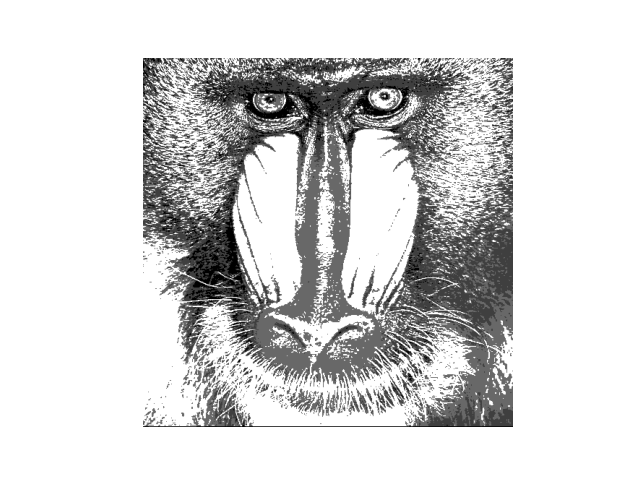
\includegraphics[width=\textwidth]{PSO_1.png}
		\caption{Case1}%注释1.jpg
		\end{minipage}
	\begin{minipage}[t]{0.2\textwidth}
		\centering
		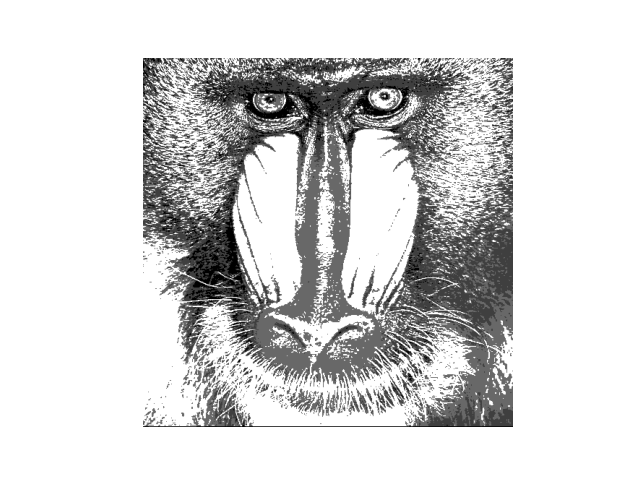
\includegraphics[width=\textwidth]{PSO_2.png}
		\caption{Case2}
	\end{minipage}
	\begin{minipage}[t]{0.2\textwidth}
		\centering
		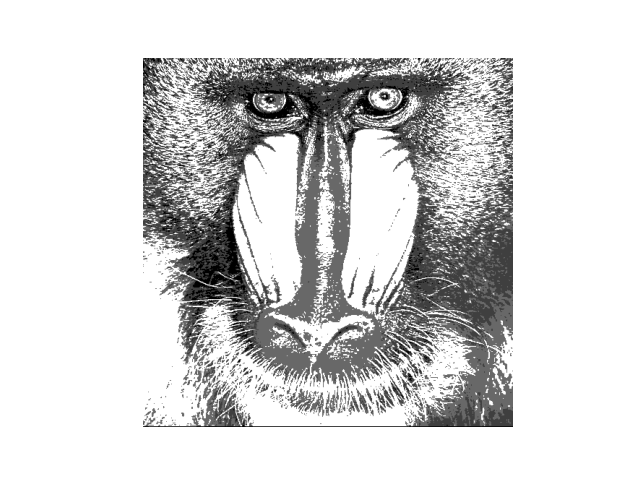
\includegraphics[width=\textwidth]{PSO_3.png}
		\caption{Case3}
	\end{minipage}
	\begin{minipage}[t]{0.2\textwidth}
		\centering
		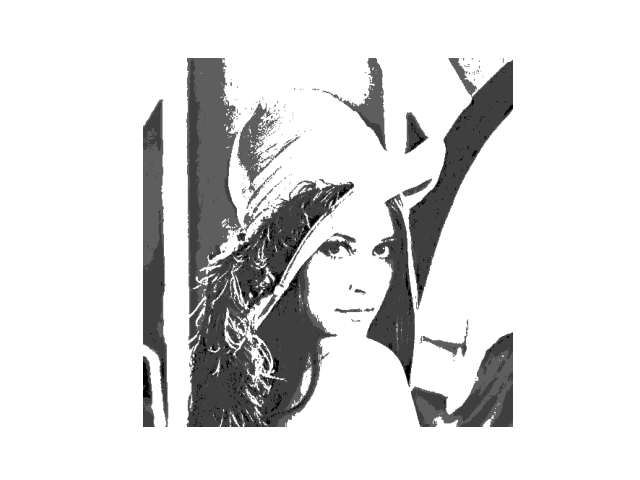
\includegraphics[width=\textwidth]{PSO_4.png}
		\caption{Case4}
	\end{minipage}
	\begin{minipage}[t]{0.2\textwidth}
		\centering
		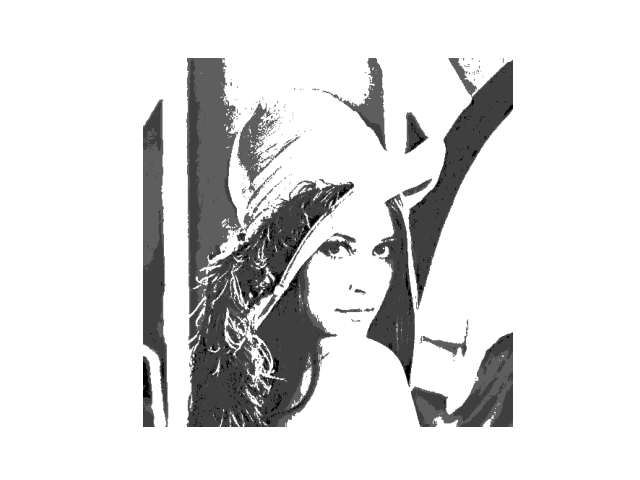
\includegraphics[width=\textwidth]{PSO_5.png}
		\caption{Case5}
	\end{minipage}
\end{figure*}

利用粒子群算法求解OTSU多阈值问题,同样能够很快得到结果,大大减少多阈值OTSU遍历全部阈值数组所需要的时间。虽然粒子群算法也是随机算法,但由于当粒子群中的粒子汇聚在一起之后(达到局部最优点),它们不会再分离,因此粒子群算法的结果比较稳定。

\subsection{对比五种算法}
我们对设计的K-Means、FCM、SCA、GA、PSO五种图像分割算法进行实验,分别在Lenna、Baboon、Pepper三张图片上分别探究其分割效果。

实验中我们控制超参数聚类数目k=4,SCA、GA、PSO的超参数与上文保持一致。K-means和FCM能得到稳定的结果,而SCA、GA、PSO三个随机智能搜索算法,我们选取多次实验中最好的结果。五种算法的结果对比如下所示:

%-------------------------------------------------

\begin{table}[h]
	\centering
	\begin{tabular}{  c  c  c  c  c  c }
	  \hline
	  Origial Image & K-means & FCM & SCA & GA & PSO \\ \hline
	  \begin{minipage}[b]{0.08\columnwidth}
		  \centering
		  \raisebox{-.6\height}{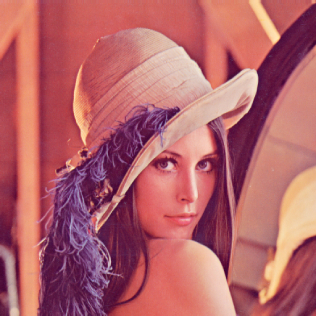
\includegraphics[width=\linewidth]{Lenna.jpg}}
	  \end{minipage}
	  & 
	  \begin{minipage}[b]{0.15\columnwidth}
		\centering
		\raisebox{-.6\height}{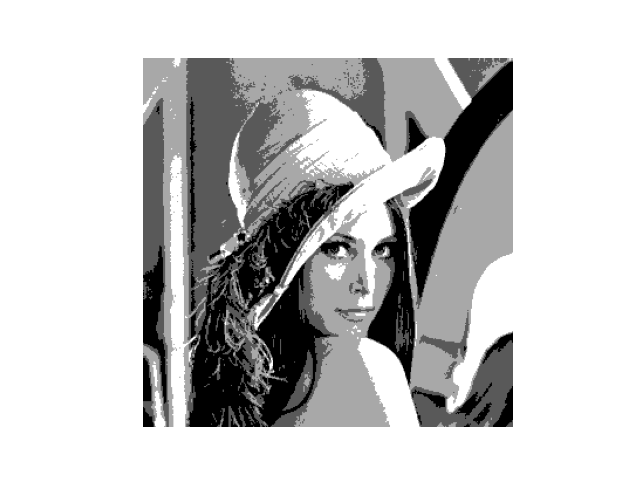
\includegraphics[width=\linewidth]{K-means_2.png}}
	  \end{minipage}
	  & 
	  \begin{minipage}[b]{0.15\columnwidth}
		\centering
		\raisebox{-.6\height}{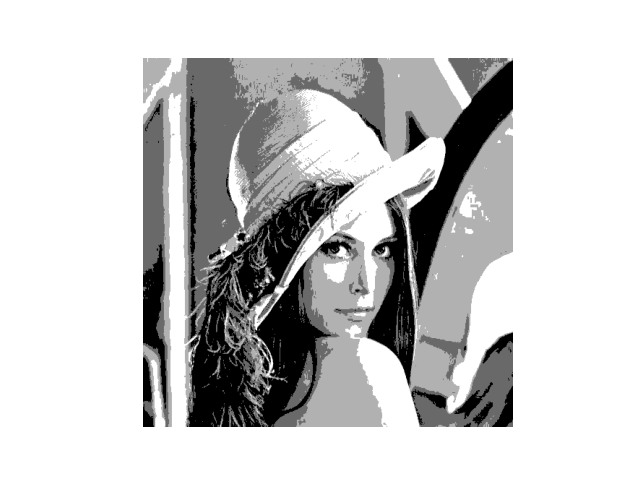
\includegraphics[width=\linewidth]{FCM_Lena.png}}
	  \end{minipage}
	  &
	  \begin{minipage}[b]{0.15\columnwidth}
		\centering
		\raisebox{-.6\height}{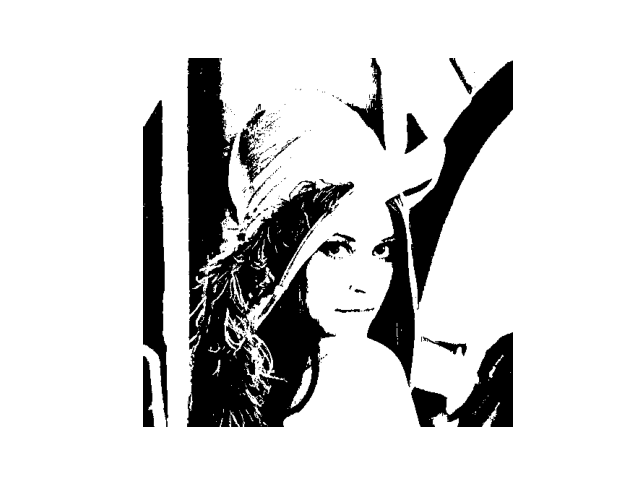
\includegraphics[width=\linewidth]{SCA2_Lena.png}}
	  \end{minipage}
	  &
	  \begin{minipage}[b]{0.15\columnwidth}
		\centering
		\raisebox{-.6\height}{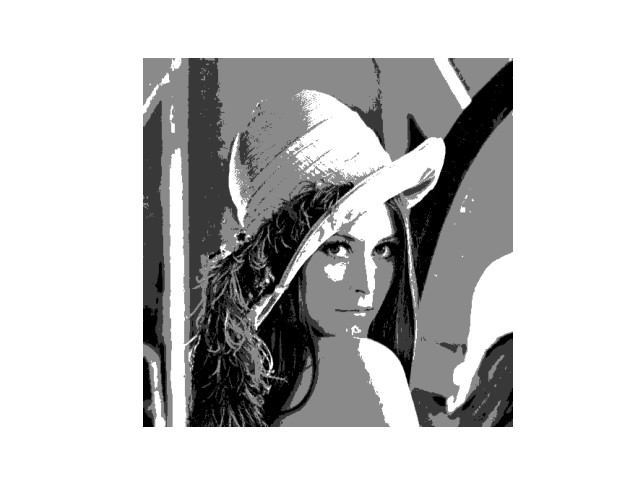
\includegraphics[width=\linewidth]{GA_Lena3.png}}
	  \end{minipage}	
	  & 
	  \begin{minipage}[b]{0.15\columnwidth}
		\centering
		\raisebox{-.6\height}{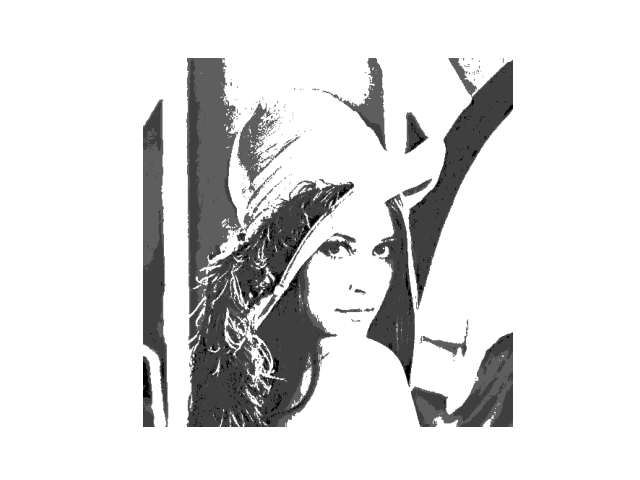
\includegraphics[width=\linewidth]{PSO_Lena2.png}}
	  \end{minipage}	   
	  \\ \hline
%-------------------------------------------------
	\begin{minipage}[b]{0.08\columnwidth}
		\centering
		\raisebox{-.6\height}{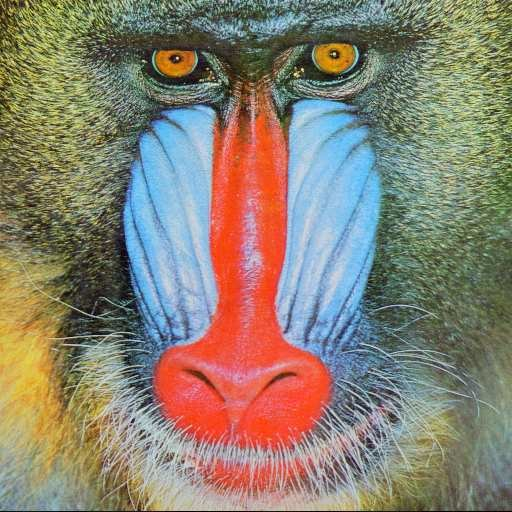
\includegraphics[width=\linewidth]{photo2.png}}
	\end{minipage}
	& 
	\begin{minipage}[b]{0.15\columnwidth}
	\centering
	\raisebox{-.6\height}{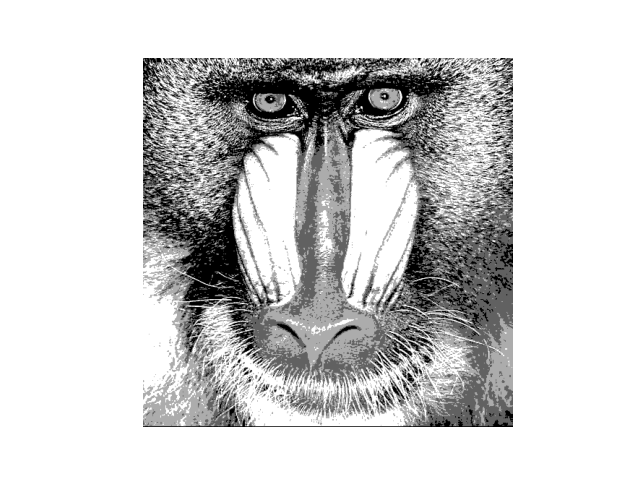
\includegraphics[width=\linewidth]{K-means_Baboon.png}}
	\end{minipage}
	& 
	\begin{minipage}[b]{0.15\columnwidth}
	\centering
	\raisebox{-.6\height}{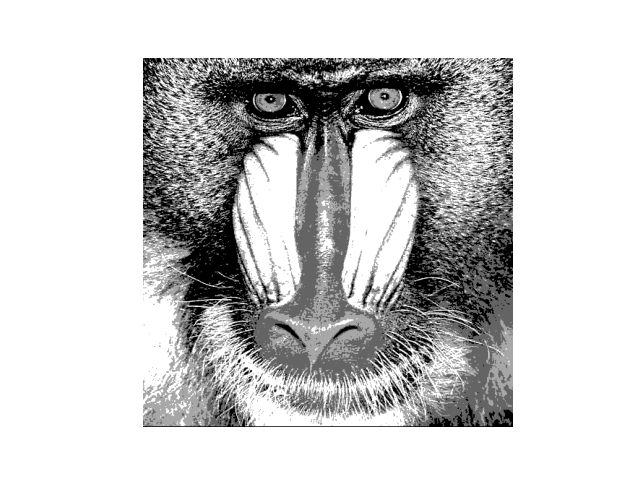
\includegraphics[width=\linewidth]{FCM_Baboon.png}}
	\end{minipage}
	&
	\begin{minipage}[b]{0.15\columnwidth}
	\centering
	\raisebox{-.6\height}{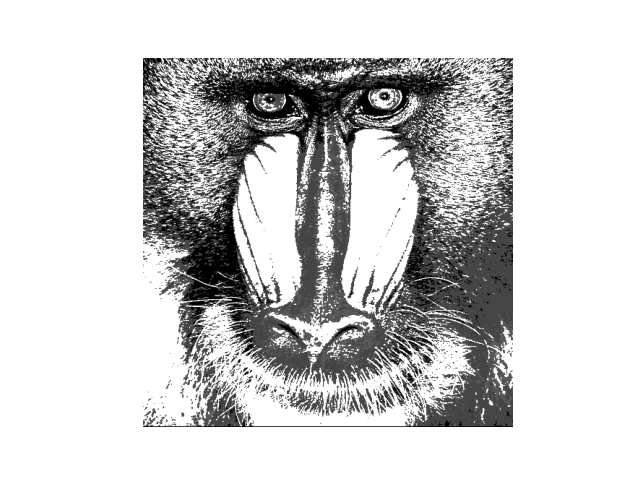
\includegraphics[width=\linewidth]{SCA_Baboon2.png}}
	\end{minipage}
	&
	\begin{minipage}[b]{0.15\columnwidth}
	\centering
	\raisebox{-.6\height}{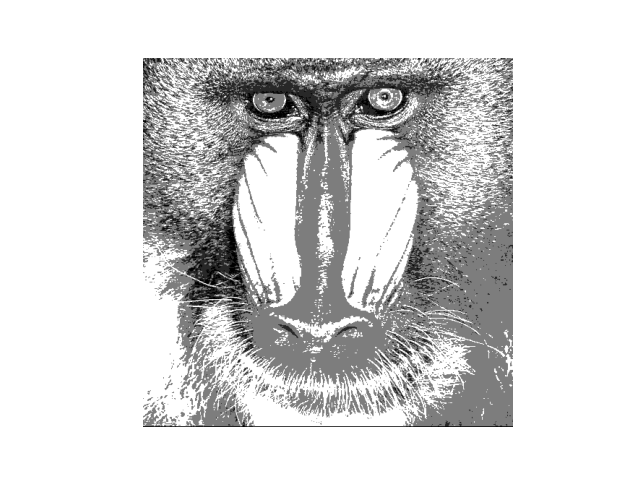
\includegraphics[width=\linewidth]{GA_Baboon.png}}
	\end{minipage}	
	& 
	\begin{minipage}[b]{0.15\columnwidth}
	\centering
	\raisebox{-.6\height}{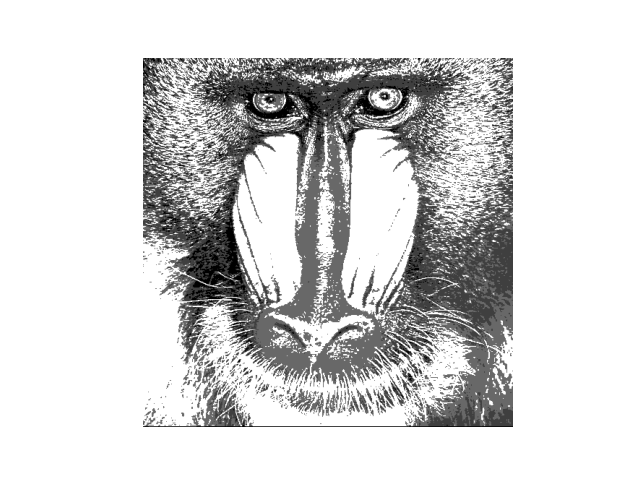
\includegraphics[width=\linewidth]{PSO_Baboon.png}}
	\end{minipage}	   
	\\ \hline
%-------------------------------------------------
	\begin{minipage}[b]{0.08\columnwidth}
		\centering
		\raisebox{-.6\height}{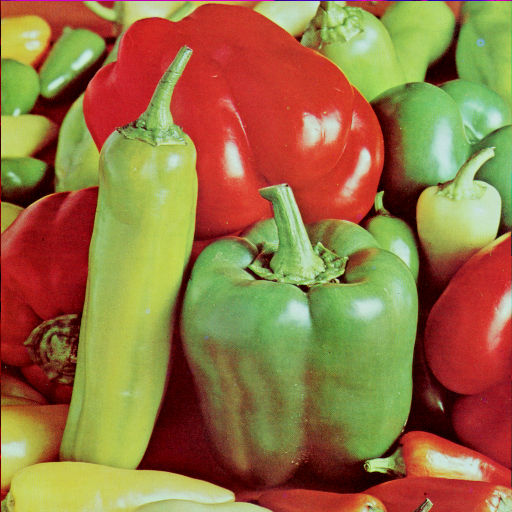
\includegraphics[width=\linewidth]{photo3.png}}
	\end{minipage}
	& 
	\begin{minipage}[b]{0.15\columnwidth}
	\centering
	\raisebox{-.6\height}{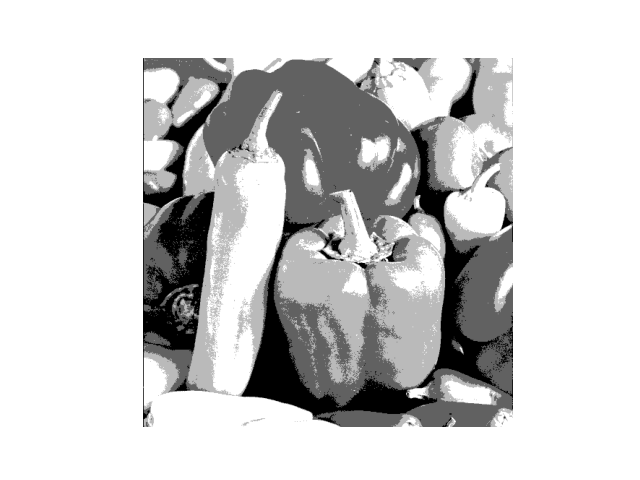
\includegraphics[width=\linewidth]{K-means_pepper.png}}
	\end{minipage}
	& 
	\begin{minipage}[b]{0.15\columnwidth}
	\centering
	\raisebox{-.6\height}{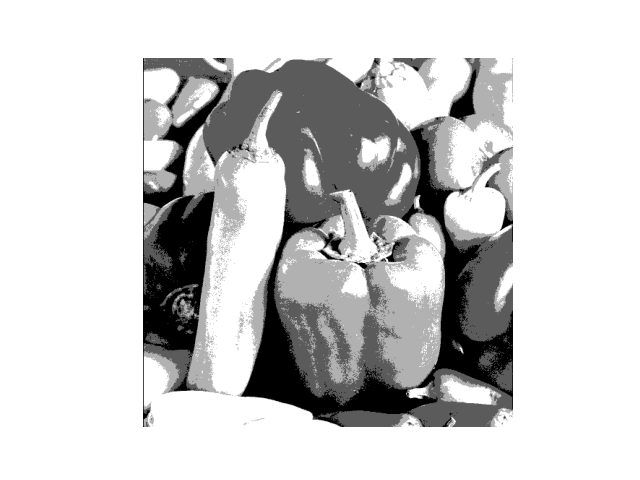
\includegraphics[width=\linewidth]{FCM_pepper.png}}
	\end{minipage}
	&
	\begin{minipage}[b]{0.15\columnwidth}
	\centering
	\raisebox{-.6\height}{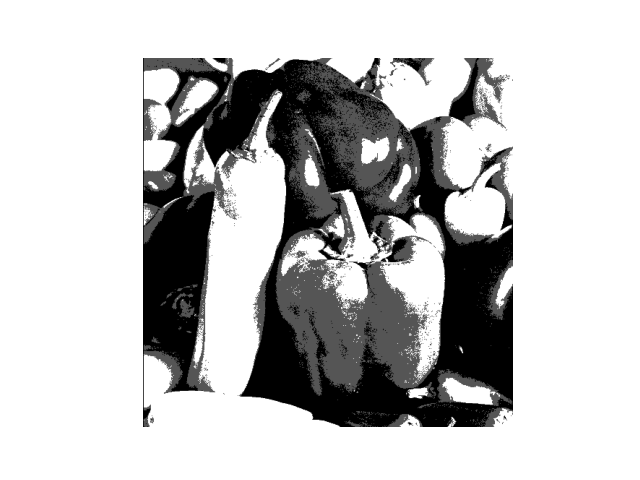
\includegraphics[width=\linewidth]{SCA_pepper.png}}
	\end{minipage}
	&
	\begin{minipage}[b]{0.15\columnwidth}
	\centering
	\raisebox{-.6\height}{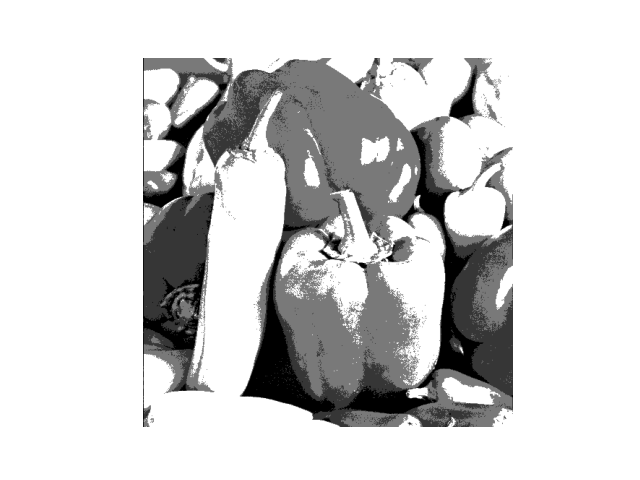
\includegraphics[width=\linewidth]{GA_pepper2.png}}
	\end{minipage}	
	& 
	\begin{minipage}[b]{0.15\columnwidth}
	\centering
	\raisebox{-.6\height}{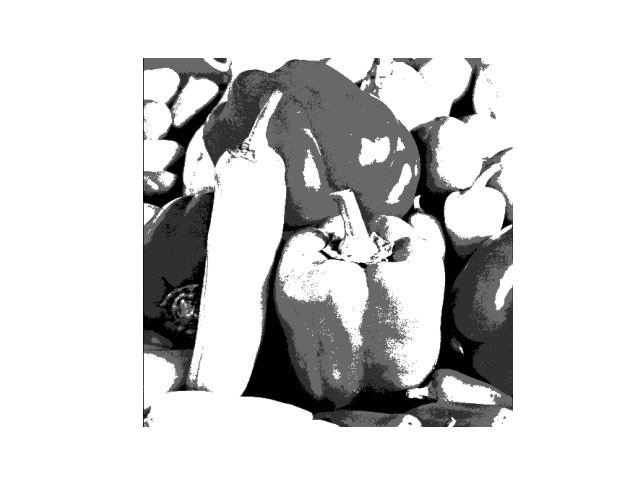
\includegraphics[width=\linewidth]{PSO_pepper.png}}
	\end{minipage}	   
	\\ \hline	

	\end{tabular}
	\caption{Image segmentation results by the diferent clustering algorithms}
\end{table}

对比五种算法,我们发现,K-means和FCM算法的结果稳定且效果最好;SCA算法的结果对比更加明显,但丧失了很多细节;GA与PSO算法的结果较好,能明显看出原图的轮廓,但细节处不如K-means和FCM算法。

另外,我们还发现我们的实验结果与论文[1]中的结果不相符。论文中K-means和FCM的效果较差,GA、PSO、SCA效果较好,其中SCA算法效果最好。而在我们的算法里,综合来看,K-means表现最好,SCA反而表现最差。

\section*{三、GUI}
\section{GUI图形界面}
\subsection{概述}

GUI图形界面是一种人与计算机通信的界面显示格式,允许用户使用鼠标等输入设备操纵屏幕上的图标或菜单选项,以选择命令、调用文件、启动程序或执行其它一些日常任务。在此次实验中,我们希望设计一个界面将代码调用和图像结果输出的部分包装起来,使可视化结果清晰明确。在Python中有多个相关的模块可供选择,我们选择使用PySide6实现GUI。

\subsection{界面设计}

我们使用Qt Designer进行界面设计。Qt Designer是一个图形化的UI设计工具,可以在PySide6的目录下找到(designer.exe),同时在Qt Creator IDE里也可以找到。

我们使用标签(Label)、按钮(Button)等模块组成界面上基本的部分,使用弹簧(Spacer)模块进行界面的空间整合。注意到Qt Designer中没有画布模块,我们将未填充文字的标签放大代替画布,并将其背景颜色设置为灰色。设计后的界面如下图所示。

\begin{figure}[H]  
	\centering
	\includegraphics[scale=0.5]{GUi界面.png}
\end{figure}

界面设计完成后,Qt Designer自动生成一个demo.ui文件,在对应环境下输入命令“PySide6-uic demo.ui -o ui$\_$demo.py”,即可生成对应的Python文件。	

\subsection{功能实现}
\subsubsection{初始化主窗口}
\begin{python}
	def __init__(self) -> None:
	super(MainWindow, self).__init__()
	self.ui = Ui_MainWindow() # UI类的实例化
	self.ui.setupUi(self)
	self.ori_img = None # 输入的原始图像
	self.dir = None # 输入图像的url地址
	self.is_ori = False # 是否已输入原始图像
	self.k = 2 # 图像分割类别数
	self.bind() # 绑定信号与槽
\end{python}

\subsubsection{绑定信号与槽}
\begin{python}
	def bind(self):
	self.ui.input_image.clicked.connect(self.origin_input) # 点击输入图像按钮,选择原始图像
	self.ui.output_image.clicked.connect(self.output) # 点击生成图像按钮,生成聚类后的图像
\end{python}

\subsubsection{图像的输入与输出}
\begin{python}
	def origin_input(self):
	dir = QMainWindow()
	file_choose = QFileDialog(dir)
	file_dir = file_choose.getOpenFileName(dir, "原始图像", "", "*.png;;*.jpg;;All Files(*)") # 输入图片地址
	self.dir = file_dir[0]
	self.ori_img = cv2.imread(self.dir, cv2.IMREAD_GRAYSCALE)
	self.ui.Origin_image.setStyleSheet(f"border-image: url({file_dir[0]});") # 输出原始图像
	self.is_ori = True
	
	def output(self):
	if self.ui.k_value.value() >= 2: # 若k>=2,则使用输入的k,否则使用缺省值k=4
	self.k = self.ui.k_value.value()
	if self.ui.Kmeans_box.isChecked():
	self.output_kmeans()
	if self.ui.FCM_box.isChecked():
	self.output_FCM()
	if self.ui.GA_box.isChecked():
	self.output_GA()
	if self.ui.PSO_box.isChecked():
	self.output_PSO()
	if self.ui.SCA_box.isChecked():
	self.output_SCA()
\end{python}

\subsubsection{对应算法的实现}
\begin{python}
	# 以K-means为例,其余类似
	def output_kmeans(self):
	if self.is_ori: # 若无输入图像,则无法生成图像
	Kmeans_img = Image.open(self.dir).convert('L')
	Kmeans_img = np.array(Kmeans_img, dtype='int32')
	Kmeans_img = np.expand_dims(Kmeans_img, axis=2)
	Kmeans_img = k_means(Kmeans_img, k=self.k)
	Kmeans_img = np.squeeze(Kmeans_img, axis=2)
	Kmeans_img = np.array(Kmeans_img, dtype='uint8')
	Kmeans_img = Image.fromarray(Kmeans_img)
	Kmeans_img = Kmeans_img.toqpixmap()
	Kmeans_img = Kmeans_img.scaledToHeight(self.ui.Kmeans_image.height())
	Kmeans_img = Kmeans_img.scaledToWidth(self.ui.Kmeans_image.width())
	self.ui.Kmeans_image.setPixmap(Kmeans_img)
\end{python}

\section*{参考文献}
[1]Lahbib Khrissi, Nabil El Akkad, Hassan Satori, 
Khalid Satori, Clustering method and sine cosine algorithm for image segmentation, Evolutionary Intelligence (2022) 15:669–682 

[2]Zhao L T, Zeng G R, He L Y, et al. Forecasting short-term oil price with a generalised pattern matching model based on empirical genetic algorithm[J]. Computational Economics, 2020, 55(4): 1151-1169.

\section*{小组分工}
\textbf{李裕硕:}k-means算法代码及报告,SCA算法代码,GA算法代码,PSO算法代码,实验结果与讨论报告

\textbf{朱宇玄:}FCM算法优化代码,GA算法优化报告,GUI界面的实现,GUI工作手册

\textbf{卞婧贤:}GMM算法代码及报告,FCM算法代码及报告,SCA算法报告,GA算法报告,PSO算法报告

\textbf{开发环境:}Pycharm
\end{document}